La grafica vettoriale \`e una tecnica utilizzata in computer grafica per descrivere 
un'immagine. 
Un' immagine \`e descritta mediante un insieme di primitive geometriche che definiscono punti, linee, curve e poligoni ai quali possono essere attribuiti colori e anche sfumature. La grafica vettoriale presenta  vantaggi rispettio alla grafica raster\footnote{La grafica raster, o bitmap, \`e una tecnica per descrivere un'immagine digitale. \`E radicalmente diversa rispetto alla grafica vettoriale in quanto l’immagine \`e composta da una griglia di punti detti pixel, di forma quadrata.}; i principali vantaggi sono:
\begin{itemize}
\item possibilit\`a di esprimere i dati in una forma direttamente comprensibile ad un essere umano;
\item possibilit\`a di esprimere i dati in un formato che occupi (molto) meno spazio rispetto all'equivalente raster;
\item possibilit\`a di ingrandire l'immagine arbitrariamente, senza che si verifichi una perdita di risoluzione dell'immagine stessa.
\end{itemize}
\begin{figure}[!htb]
\centering%
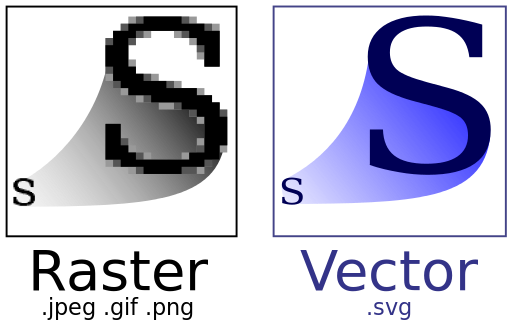
\includegraphics[scale=0.4]{Vect.png}%
\caption{Differenza fra immagine di tipo raster e vettoriale.}\label{fig:imgVet}%
\end{figure}
\subsection{Scalable Vector Graphics}
Scalable Vector Graphics abbreviato in SVG, indica una tecnologia in grado di visualizzare oggetti di grafica vettoriale e, pertanto, di gestire immagini scalabili dimensionalmente.
Più specificamente si tratta di un linguaggio derivato dall'XML, cioè di un'applicazione del metalinguaggio posto a base degli sviluppi del Web da parte del consorzio W3C, che si pone l'obiettivo di descrivere figure bidimensionali statiche e animate.
Vediamo di elencare brevemente quelle che sono le caratteristiche principali di SVG:
\begin{description}
\item[È testuale:]questo implica che è possibile creare e modificare un file SVG con un semplicissimo editor di testo; inoltre si ha la possibilità di comprimere un file testuale in maniera molto efficiente favorendo così l’utilizzo di SVG in ambito Web;
\item[È vettoriale:]questo implica che, a differenza di quello che avviene nel caso di un formato grafico raster (Jpeg o Gif), è possibile scalare e zoommare a piacimento l’immagine SVG senza avere una perdita di qualità dell’immagine stessa;
\item[È open:]non è un formato proprietario, le specifiche ed i lavori del Working Group che si occupa di SVG sono liberamente consultabili sul sito del W3C;
\item[È un’applicazione XML:]questo permette di utilizzare, per lo sviluppo di applicazioni che manipolano file SVG, i numerosi strumenti di sviluppo già esistenti per XML;
\item[È interattivo:]attraverso un linguaggio di scripting è possibile rendere l’immagine SVG interattiva, ossia fare in modo che sia sensibile a certi eventi (come il click del mouse) e che compia determinate azioni in risposta a tali eventi;
\item[È dinamico:]infatti è possibile creare delle animazioni attraverso l’uso del linguaggio di animazione SMIL (Synchronized Multimedia Integration Language) anch’esso sviluppato dal W3C.
\end{description}

Gli oggetti grafici possono essere raggruppati in oggetti più comprensivi, muniti di attributi di stile e aggiunti ad oggetti grafici precedentemente costruiti e visualizzati. Un testo può far parte di un qualsiasi namespace XML sottoponibile ad una applicazione; questa possibilità consente di aumentare la ricercabilità e l'accessibilità delle immagini SVG.
Due programmi di grafica vettoriale open source e multipiattaforma che usano in maniera nativa il formato SVG sono Inkscape e Sodipodi.
Nel progetto sono è stata utilizzata la versione 1.1 di SVG per la compatibilità con le librerie utilizzate.